% Options for packages loaded elsewhere
\PassOptionsToPackage{unicode}{hyperref}
\PassOptionsToPackage{hyphens}{url}
%
\documentclass[
]{article}
\usepackage{amsmath,amssymb}
\usepackage{lmodern}
\usepackage{ifxetex,ifluatex}
\ifnum 0\ifxetex 1\fi\ifluatex 1\fi=0 % if pdftex
  \usepackage[T1]{fontenc}
  \usepackage[utf8]{inputenc}
  \usepackage{textcomp} % provide euro and other symbols
\else % if luatex or xetex
  \usepackage{unicode-math}
  \defaultfontfeatures{Scale=MatchLowercase}
  \defaultfontfeatures[\rmfamily]{Ligatures=TeX,Scale=1}
\fi
% Use upquote if available, for straight quotes in verbatim environments
\IfFileExists{upquote.sty}{\usepackage{upquote}}{}
\IfFileExists{microtype.sty}{% use microtype if available
  \usepackage[]{microtype}
  \UseMicrotypeSet[protrusion]{basicmath} % disable protrusion for tt fonts
}{}
\makeatletter
\@ifundefined{KOMAClassName}{% if non-KOMA class
  \IfFileExists{parskip.sty}{%
    \usepackage{parskip}
  }{% else
    \setlength{\parindent}{0pt}
    \setlength{\parskip}{6pt plus 2pt minus 1pt}}
}{% if KOMA class
  \KOMAoptions{parskip=half}}
\makeatother
\usepackage{xcolor}
\IfFileExists{xurl.sty}{\usepackage{xurl}}{} % add URL line breaks if available
\IfFileExists{bookmark.sty}{\usepackage{bookmark}}{\usepackage{hyperref}}
\hypersetup{
  pdftitle={Visualizations with statistical details: The `ggstatsplot' approach},
  hidelinks,
  pdfcreator={LaTeX via pandoc}}
\urlstyle{same} % disable monospaced font for URLs
\usepackage[margin=1in]{geometry}
\usepackage{color}
\usepackage{fancyvrb}
\newcommand{\VerbBar}{|}
\newcommand{\VERB}{\Verb[commandchars=\\\{\}]}
\DefineVerbatimEnvironment{Highlighting}{Verbatim}{commandchars=\\\{\}}
% Add ',fontsize=\small' for more characters per line
\usepackage{framed}
\definecolor{shadecolor}{RGB}{248,248,248}
\newenvironment{Shaded}{\begin{snugshade}}{\end{snugshade}}
\newcommand{\AlertTok}[1]{\textcolor[rgb]{0.94,0.16,0.16}{#1}}
\newcommand{\AnnotationTok}[1]{\textcolor[rgb]{0.56,0.35,0.01}{\textbf{\textit{#1}}}}
\newcommand{\AttributeTok}[1]{\textcolor[rgb]{0.77,0.63,0.00}{#1}}
\newcommand{\BaseNTok}[1]{\textcolor[rgb]{0.00,0.00,0.81}{#1}}
\newcommand{\BuiltInTok}[1]{#1}
\newcommand{\CharTok}[1]{\textcolor[rgb]{0.31,0.60,0.02}{#1}}
\newcommand{\CommentTok}[1]{\textcolor[rgb]{0.56,0.35,0.01}{\textit{#1}}}
\newcommand{\CommentVarTok}[1]{\textcolor[rgb]{0.56,0.35,0.01}{\textbf{\textit{#1}}}}
\newcommand{\ConstantTok}[1]{\textcolor[rgb]{0.00,0.00,0.00}{#1}}
\newcommand{\ControlFlowTok}[1]{\textcolor[rgb]{0.13,0.29,0.53}{\textbf{#1}}}
\newcommand{\DataTypeTok}[1]{\textcolor[rgb]{0.13,0.29,0.53}{#1}}
\newcommand{\DecValTok}[1]{\textcolor[rgb]{0.00,0.00,0.81}{#1}}
\newcommand{\DocumentationTok}[1]{\textcolor[rgb]{0.56,0.35,0.01}{\textbf{\textit{#1}}}}
\newcommand{\ErrorTok}[1]{\textcolor[rgb]{0.64,0.00,0.00}{\textbf{#1}}}
\newcommand{\ExtensionTok}[1]{#1}
\newcommand{\FloatTok}[1]{\textcolor[rgb]{0.00,0.00,0.81}{#1}}
\newcommand{\FunctionTok}[1]{\textcolor[rgb]{0.00,0.00,0.00}{#1}}
\newcommand{\ImportTok}[1]{#1}
\newcommand{\InformationTok}[1]{\textcolor[rgb]{0.56,0.35,0.01}{\textbf{\textit{#1}}}}
\newcommand{\KeywordTok}[1]{\textcolor[rgb]{0.13,0.29,0.53}{\textbf{#1}}}
\newcommand{\NormalTok}[1]{#1}
\newcommand{\OperatorTok}[1]{\textcolor[rgb]{0.81,0.36,0.00}{\textbf{#1}}}
\newcommand{\OtherTok}[1]{\textcolor[rgb]{0.56,0.35,0.01}{#1}}
\newcommand{\PreprocessorTok}[1]{\textcolor[rgb]{0.56,0.35,0.01}{\textit{#1}}}
\newcommand{\RegionMarkerTok}[1]{#1}
\newcommand{\SpecialCharTok}[1]{\textcolor[rgb]{0.00,0.00,0.00}{#1}}
\newcommand{\SpecialStringTok}[1]{\textcolor[rgb]{0.31,0.60,0.02}{#1}}
\newcommand{\StringTok}[1]{\textcolor[rgb]{0.31,0.60,0.02}{#1}}
\newcommand{\VariableTok}[1]{\textcolor[rgb]{0.00,0.00,0.00}{#1}}
\newcommand{\VerbatimStringTok}[1]{\textcolor[rgb]{0.31,0.60,0.02}{#1}}
\newcommand{\WarningTok}[1]{\textcolor[rgb]{0.56,0.35,0.01}{\textbf{\textit{#1}}}}
\usepackage{graphicx}
\makeatletter
\def\maxwidth{\ifdim\Gin@nat@width>\linewidth\linewidth\else\Gin@nat@width\fi}
\def\maxheight{\ifdim\Gin@nat@height>\textheight\textheight\else\Gin@nat@height\fi}
\makeatother
% Scale images if necessary, so that they will not overflow the page
% margins by default, and it is still possible to overwrite the defaults
% using explicit options in \includegraphics[width, height, ...]{}
\setkeys{Gin}{width=\maxwidth,height=\maxheight,keepaspectratio}
% Set default figure placement to htbp
\makeatletter
\def\fps@figure{htbp}
\makeatother
\setlength{\emergencystretch}{3em} % prevent overfull lines
\providecommand{\tightlist}{%
  \setlength{\itemsep}{0pt}\setlength{\parskip}{0pt}}
\setcounter{secnumdepth}{-\maxdimen} % remove section numbering
\ifluatex
  \usepackage{selnolig}  % disable illegal ligatures
\fi
\newlength{\cslhangindent}
\setlength{\cslhangindent}{1.5em}
\newlength{\csllabelwidth}
\setlength{\csllabelwidth}{3em}
\newenvironment{CSLReferences}[2] % #1 hanging-ident, #2 entry spacing
 {% don't indent paragraphs
  \setlength{\parindent}{0pt}
  % turn on hanging indent if param 1 is 1
  \ifodd #1 \everypar{\setlength{\hangindent}{\cslhangindent}}\ignorespaces\fi
  % set entry spacing
  \ifnum #2 > 0
  \setlength{\parskip}{#2\baselineskip}
  \fi
 }%
 {}
\usepackage{calc}
\newcommand{\CSLBlock}[1]{#1\hfill\break}
\newcommand{\CSLLeftMargin}[1]{\parbox[t]{\csllabelwidth}{#1}}
\newcommand{\CSLRightInline}[1]{\parbox[t]{\linewidth - \csllabelwidth}{#1}\break}
\newcommand{\CSLIndent}[1]{\hspace{\cslhangindent}#1}

\title{Visualizations with statistical details: The `ggstatsplot'
approach}
\author{}
\date{\vspace{-2.5em}2021-05-24}

\begin{document}
\maketitle

\hypertarget{summary}{%
\section{Summary}\label{summary}}

Graphical displays can reveal problems in a statistical model that might
not be apparent from purely numerical summaries. Such visualizations can
also be helpful for the reader to evaluate the validity of a model if it
is reported in a scholarly publication/report. But, given the onerous
costs involved, researchers can avoid preparing information-rich
graphics and exploring several statistical approaches/tests available.
The \texttt{ggstatsplot} package in R programming language
(\protect\hyperlink{ref-base2021}{R Core Team, 2021}) provides a
one-line syntax to enrich \texttt{ggplot2}-based visualizations with the
results from statistical analysis embedded in the visualization itself.
In doing so, the package helps researchers adopt a rigorous, reliable,
and robust data exploratory and reporting workflow.

\hypertarget{statement-of-need}{%
\section{Statement of Need}\label{statement-of-need}}

In a typical data analysis workflow, data visualization and statistical
modeling are two different phases: visualization informs modeling, and
in turn, modeling can suggest a different visualization method, and so
on and so forth (\protect\hyperlink{ref-wickham2016r}{Wickham \&
Grolemund, 2016}). The central idea of \texttt{ggstatsplot} is simple:
combine these two phases into one in the form of an informative graphic
with statistical details.

Before discussing benefits of this approach, we will see one example
(Figure 1).

\begin{Shaded}
\begin{Highlighting}[]
\FunctionTok{set.seed}\NormalTok{(}\DecValTok{123}\NormalTok{) }\CommentTok{\# for reproducibility}
\FunctionTok{library}\NormalTok{(palmerpenguins) }\CommentTok{\# for \textquotesingle{}penguins\textquotesingle{} dataset}
\FunctionTok{library}\NormalTok{(ggstatsplot)}

\FunctionTok{ggbetweenstats}\NormalTok{(penguins, species, body\_mass\_g)}
\end{Highlighting}
\end{Shaded}

\begin{figure}
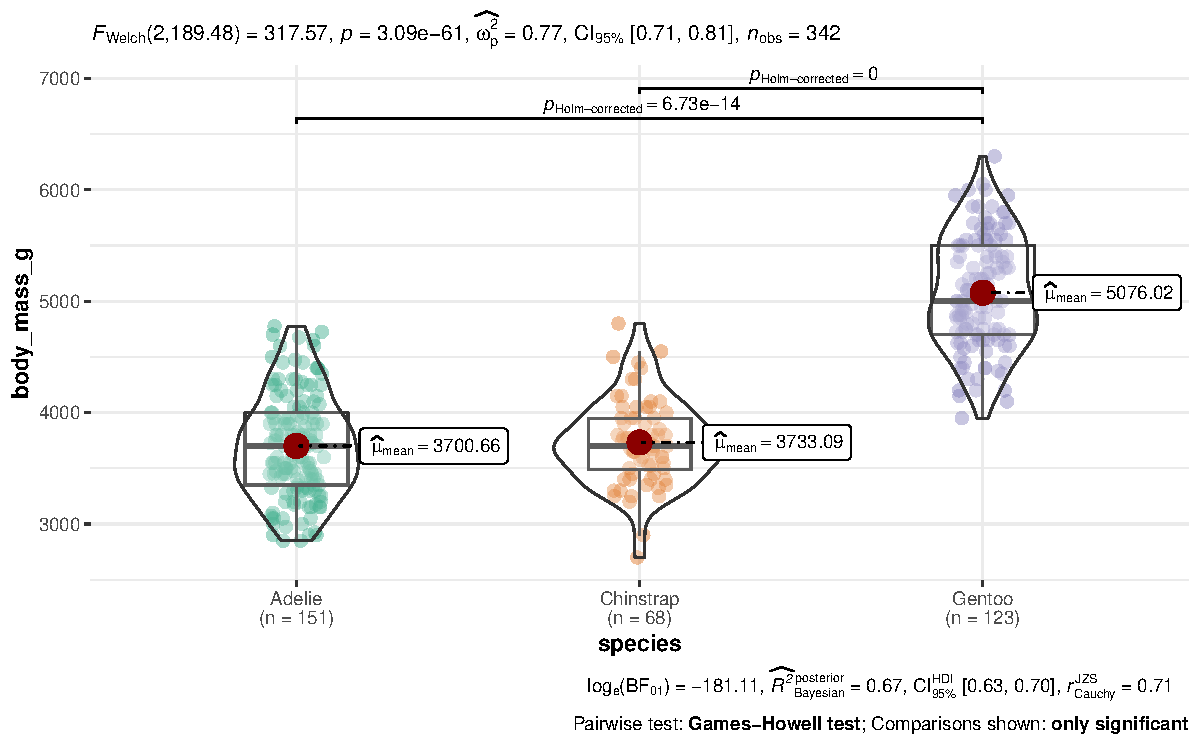
\includegraphics[width=1\linewidth]{paper_files/figure-latex/penguins-1} \caption{Example plot from the `ggstatsplot` package illustrates its philosophy of juxtaposing informative visualizations with details from statistical analysis. To see all supported plots and statistical analyses, see the package website: \url{https://indrajeetpatil.github.io/ggstatsplot/}}\label{fig:penguins}
\end{figure}

As can be seen, with a single line of code, the function produces
details about descriptive statistics, inferential statistics, effect
size estimate and its uncertainty, pairwise comparisons, Bayesian
hypothesis testing, Bayesian posterior estimate and its uncertainty.
Moreover, these details are juxtaposed with informative and well-labeled
visualizations. The defaults are designed to follow best practices in
both data visualization
(\protect\hyperlink{ref-cleveland1985}{Cleveland, 1985};
\protect\hyperlink{ref-grant2018data}{Grant, 2018};
\protect\hyperlink{ref-healy2018data}{Healy, 2018};
\protect\hyperlink{ref-tufte2001}{Tufte, 2001};
\protect\hyperlink{ref-wilke2019fundamentals}{Wilke, 2019}) and
(Frequentist/Bayesian) statistical reporting
(\protect\hyperlink{ref-apa2019}{American Psychological Association,
2019}; \protect\hyperlink{ref-van2020jasp}{Doorn et al., 2020}). Without
\texttt{ggstatsplot}, getting these statistical details and customizing
a plot would require significant amount of time and effort In other
words, this package removes the trade-off often faced by researchers
between ease and thoroughness of data exploration and further cements
good data exploration habits.

Internally, data cleaning is carried out using \texttt{tidyverse}
(\protect\hyperlink{ref-Wickham2019}{Wickham et al., 2019}), while
statistical analysis is carried out via \texttt{statsExpressions}
(\protect\hyperlink{ref-Patil2021}{Indrajeet Patil, 2021}) and
\texttt{easystats} (\protect\hyperlink{ref-Ben-Shachar2020}{Ben-Shachar,
Lüdecke, \& Makowski, 2020};
\protect\hyperlink{ref-Luxfcdecke2020parameters}{Lüdecke, Ben-Shachar,
Patil, \& Makowski, 2020};
\protect\hyperlink{ref-Luxfcdecke2020performance}{Lüdecke, Ben-Shachar,
Patil, Waggoner, \& Makowski, 2021};
\protect\hyperlink{ref-Luxfcdecke2019}{Lüdecke, Waggoner, \& Makowski,
2019}; \protect\hyperlink{ref-Makowski2019}{Makowski, Ben-Shachar, \&
Lüdecke, 2019}; \protect\hyperlink{ref-Makowski2020}{Makowski,
Ben-Shachar, Patil, \& Lüdecke, 2020}) packages. All visualizations are
constructed using the grammar of graphics framework
(\protect\hyperlink{ref-Wilkinson2012}{Wilkinson, 2012}), as implemented
in the \texttt{ggplot2} package
(\protect\hyperlink{ref-Wickham2016}{Wickham, 2016}).

\hypertarget{benefits}{%
\section{Benefits}\label{benefits}}

In summary, the benefits of \texttt{ggstatsplot}'s approach are the
following. It-

\begin{enumerate}
\def\labelenumi{\alph{enumi}.}
\item
  produces charts displaying both raw data, and numerical plus graphical
  summary indices,
\item
  avoids errors in and increases reproducibility of statistical
  reporting,
\item
  highlights the importance of the effect by providing effect size
  measures by default,
\item
  provides an easy way to evaluate \emph{absence} of an effect using
  Bayes factors,
\item
  encourages researchers and readers to evaluate statistical assumptions
  of a model in the context of the underlying data (Figure 2),
\item
  is easy and simple enough that someone with little-to-no coding
  experience can use it without making an error and may even encourage
  beginners to programmatically analyze data, instead of using GUI
  software.
\end{enumerate}

\begin{figure}
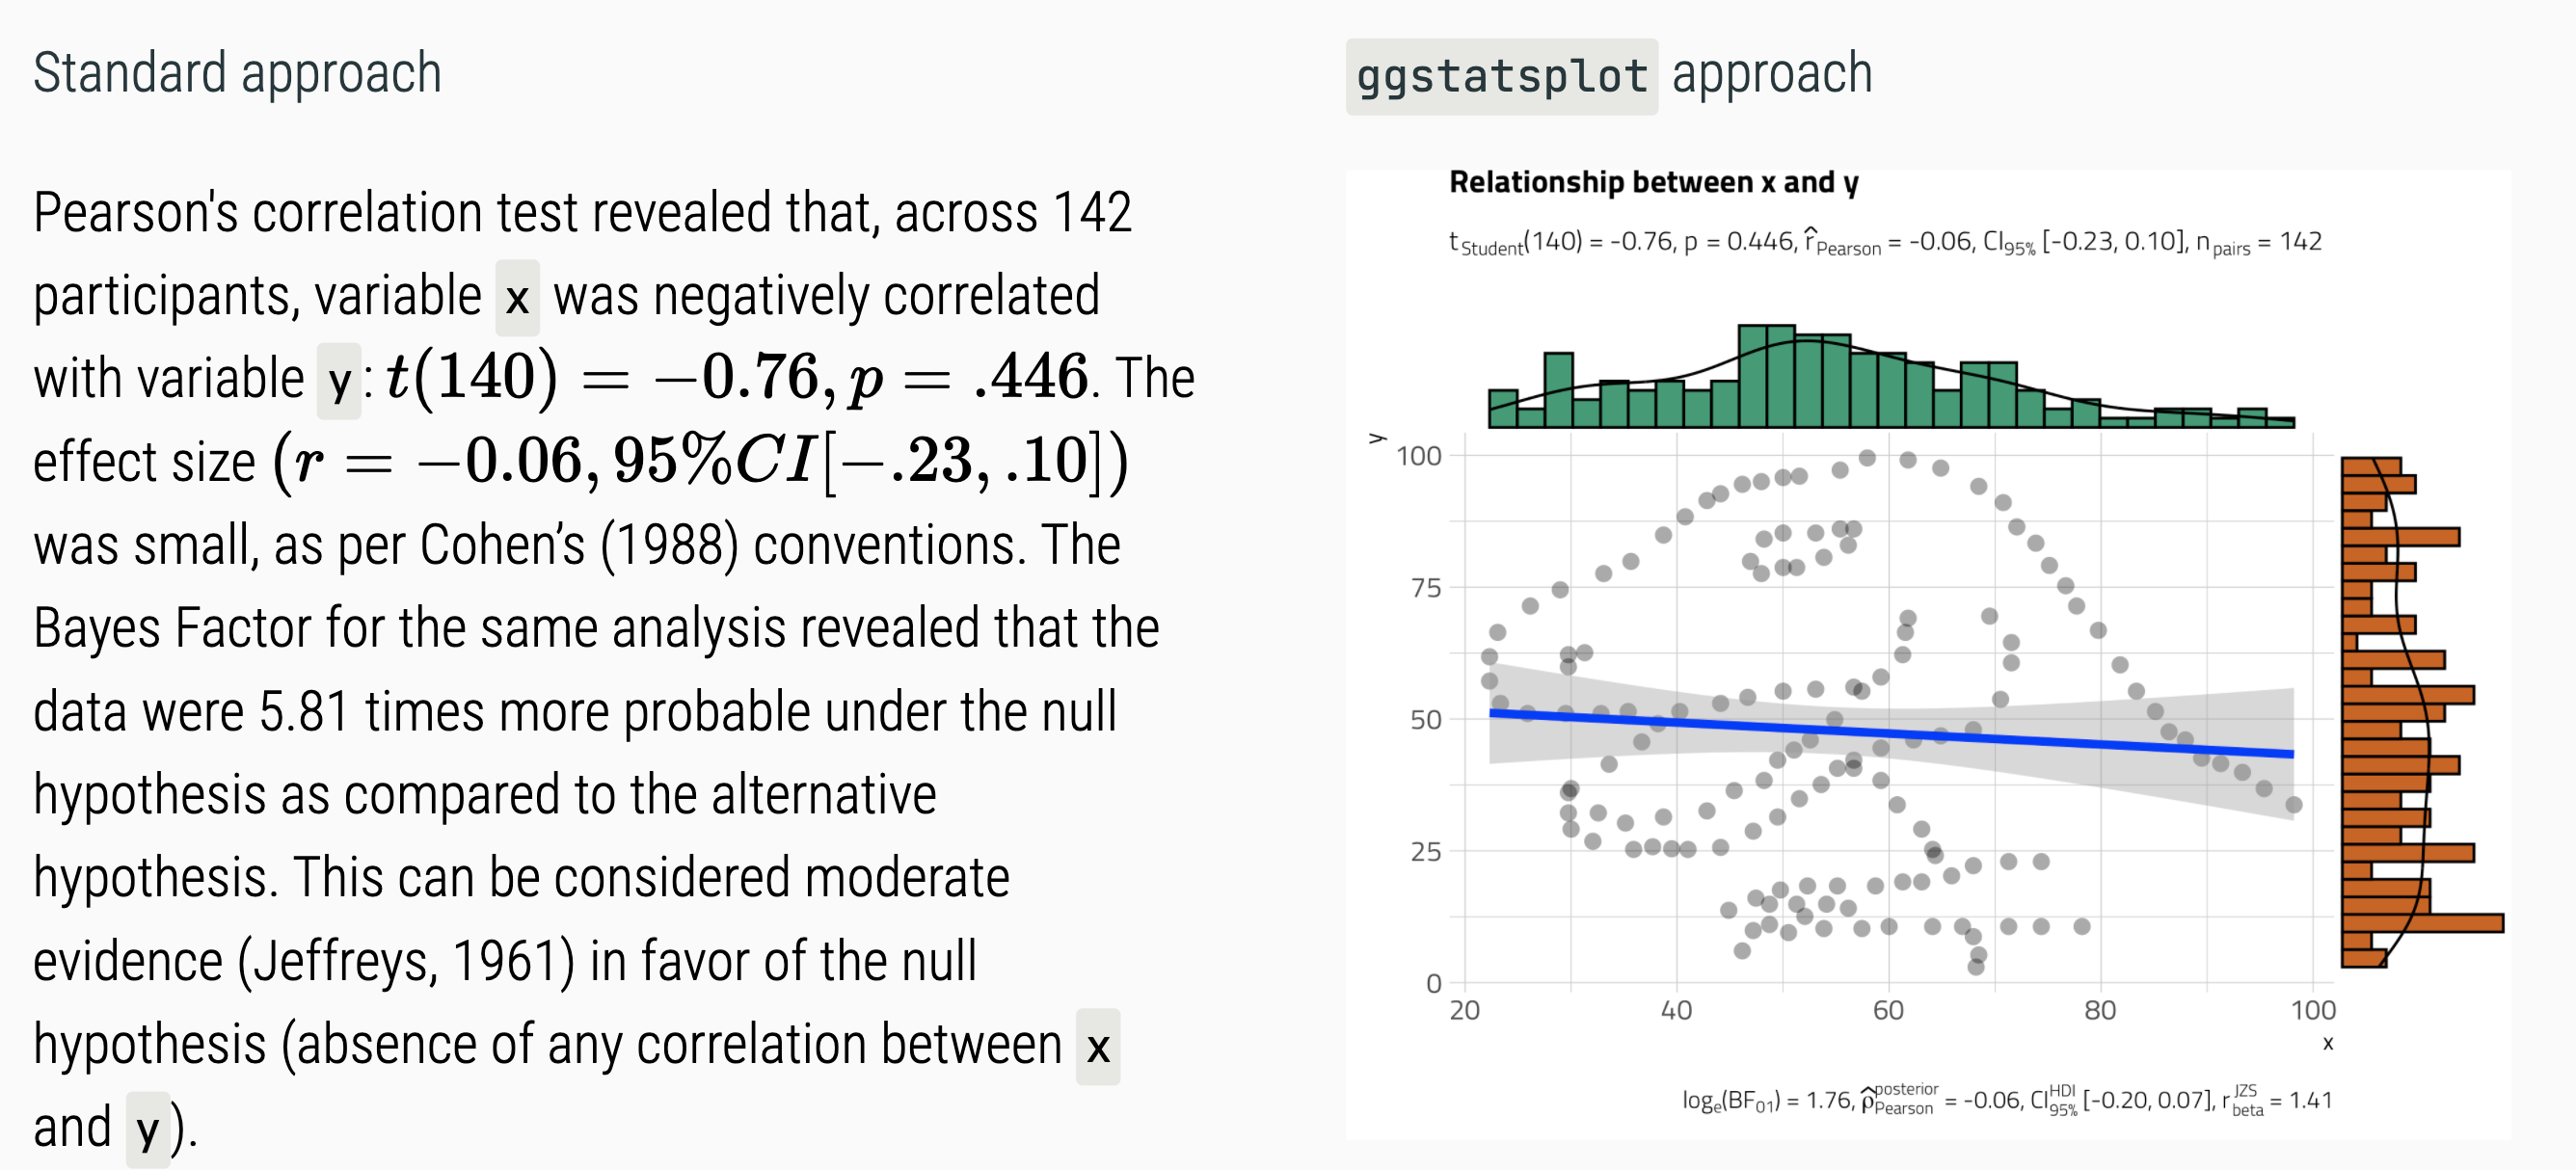
\includegraphics[width=1\linewidth]{reporting} \caption{Comparing the 'Standard' approach of reporting statistical analysis in a publication/report with the 'ggstatsplot' approach of reporting the same analysis next to an informative graphic. Note that the results described in the 'Standard' approach are about the 'Dinosaur' dataset plotted on the right. Without the accompanying visualization, it is hard to evaluate the validity of the results. The ideal reporting practice will be a hybrid of these two approaches where the plot contains both the visual and numerical summaries about a statistical model, while the narrative provides interpretative context for the reported statistics.}\label{fig:reporting}
\end{figure}

\hypertarget{future-scope}{%
\section{Future Scope}\label{future-scope}}

This package is an ambitious, ongoing, and long-term project. It
currently supports common statistical tests (parametric, non-parametric,
robust, or Bayesian \emph{t}-test, one-way ANOVA, contingency table
analysis, correlation analysis, meta-analysis, regression analyses,
etc.) and corresponding visualizations (box/violin plot, scatter plot,
dot-and-whisker plot, pie chart, bar chart, etc.). It will continue
expanding to support ever increasing collection of statistical analyses
and visualizations.

\hypertarget{licensing-and-availability}{%
\section{Licensing and Availability}\label{licensing-and-availability}}

\texttt{ggstatsplot} is licensed under the GNU General Public License
(v3.0), with all source code stored at
\href{https://github.com/IndrajeetPatil/ggstatsplot/}{GitHub}. In the
spirit of honest and open science, requests and suggestions for fixes,
feature updates, as well as general questions and concerns are
encouraged via direct interaction with contributors and developers by
filing an
\href{https://github.com/IndrajeetPatil/ggstatsplot/issues}{issue} while
respecting
\href{https://indrajeetpatil.github.io/ggstatsplot/CONTRIBUTING.html}{\emph{Contribution
Guidelines}}.

\hypertarget{acknowledgements}{%
\section{Acknowledgements}\label{acknowledgements}}

I would like to acknowledge the support of Mina Cikara, Fiery Cushman,
and Iyad Rahwan during the development of this project.
\texttt{ggstatsplot} relies heavily on the
\href{https://github.com/easystats/easystats}{\texttt{easystats}}
ecosystem, a collaborative project created to facilitate the usage of
\texttt{R} for statistical analyses. Thus, I would like to thank the
\href{https://github.com/orgs/easystats/people}{members} of
\texttt{easystats} as well as the users. I would additionally like to
thank the contributors to \texttt{ggstatsplot} for reporting bugs,
providing helpful feedback, or helping with enhancements.

\hypertarget{references}{%
\section*{References}\label{references}}
\addcontentsline{toc}{section}{References}

\hypertarget{refs}{}
\begin{CSLReferences}{1}{0}
\leavevmode\hypertarget{ref-apa2019}{}%
American Psychological Association. (2019). \emph{Publication {Manual}
of the {American Psychological Association}, 7th {Edition}}.
{Washington, DC}: {American Psychological Association}.

\leavevmode\hypertarget{ref-Ben-Shachar2020}{}%
Ben-Shachar, M. S., Lüdecke, D., \& Makowski, D. (2020). {e}ffectsize:
Estimation of effect size indices and standardized parameters.
\emph{Journal of Open Source Software}, \emph{5}(56), 2815.
doi:\href{https://doi.org/10.21105/joss.02815}{10.21105/joss.02815}

\leavevmode\hypertarget{ref-cleveland1985}{}%
Cleveland, W. S. (1985). \emph{The {Elements} of {Graphing Data}} (1st
edition.). {Monterey, Cal}: {Wadsworth, Inc.}

\leavevmode\hypertarget{ref-van2020jasp}{}%
Doorn, van, Bergh, J. van den, Böhm, D., Dablander, U., Derks, F.,
Draws, K., Etz, T., et al. (2020). The JASP guidelines for conducting
and reporting a {B}ayesian analysis. \emph{Psychonomic Bulletin \&
Review}, 1--14.
doi:\href{https://doi.org/10.3758/s13423-020-01798-5}{10.3758/s13423-020-01798-5}

\leavevmode\hypertarget{ref-grant2018data}{}%
Grant, R. (2018). \emph{{Data Visualization: Charts, Maps, and
Interactive Graphics}}. CRC Press.

\leavevmode\hypertarget{ref-healy2018data}{}%
Healy, K. (2018). \emph{{Data Visualization: A Practical Introduction}}.
Princeton University Press.

\leavevmode\hypertarget{ref-Patil2021}{}%
Indrajeet Patil. (2021). {statsExpressions: {R} Package for Tidy
Dataframes and Expressions with Statistical Details}. \emph{{Journal of
Open Source Software}}, \emph{6}(61), 3236.
doi:\href{https://doi.org/10.21105/joss.03236}{10.21105/joss.03236}

\leavevmode\hypertarget{ref-Luxfcdecke2020parameters}{}%
Lüdecke, D., Ben-Shachar, M. S., Patil, I., \& Makowski, D. (2020).
Extracting, computing and exploring the parameters of statistical models
using {R}. \emph{Journal of Open Source Software}, \emph{5}(53), 2445.
doi:\href{https://doi.org/10.21105/joss.02445}{10.21105/joss.02445}

\leavevmode\hypertarget{ref-Luxfcdecke2020performance}{}%
Lüdecke, D., Ben-Shachar, M. S., Patil, I., Waggoner, P., \& Makowski,
D. (2021). {performance}: An {R} package for assessment, comparison and
testing of statistical models. \emph{Journal of Open Source Software},
\emph{6}(60), 3139.
doi:\href{https://doi.org/10.21105/joss.03139}{10.21105/joss.03139}

\leavevmode\hypertarget{ref-Luxfcdecke2019}{}%
Lüdecke, D., Waggoner, P., \& Makowski, D. (2019). Insight: A unified
interface to access information from model objects in {R}. \emph{Journal
of Open Source Software}, \emph{4}(38), 1412.
doi:\href{https://doi.org/10.21105/joss.01412}{10.21105/joss.01412}

\leavevmode\hypertarget{ref-Makowski2019}{}%
Makowski, D., Ben-Shachar, M. S., \& Lüdecke, D. (2019). bayestestR:
Describing effects and their uncertainty, existence and significance
within the {B}ayesian framework. \emph{Journal of Open Source Software},
\emph{4}(40), 1541.
doi:\href{https://doi.org/10.21105/joss.01541}{10.21105/joss.01541}

\leavevmode\hypertarget{ref-Makowski2020}{}%
Makowski, D., Ben-Shachar, M. S., Patil, I., \& Lüdecke, D. (2020).
Methods and algorithms for correlation analysis in {R}. \emph{Journal of
Open Source Software}, \emph{5}(51), 2306.
doi:\href{https://doi.org/10.21105/joss.02306}{10.21105/joss.02306}

\leavevmode\hypertarget{ref-base2021}{}%
R Core Team. (2021). \emph{{R}: A language and environment for
statistical computing}. Vienna, Austria: R Foundation for Statistical
Computing. Retrieved from \url{https://www.R-project.org/}

\leavevmode\hypertarget{ref-tufte2001}{}%
Tufte, E. R. (2001). \emph{The {Visual Display} of {Quantitative
Information}} (2nd edition.). {Cheshire, Conn}: {Graphics Press}.

\leavevmode\hypertarget{ref-Wickham2016}{}%
Wickham, H. (2016). \emph{{ggplot2}: Elegant graphics for data
analysis}. Springer-Verlag New York.

\leavevmode\hypertarget{ref-Wickham2019}{}%
Wickham, H., Averick, M., Bryan, J., Chang, W., McGowan, L. D.,
François, R., Grolemund, G., et al. (2019). Welcome to the {tidyverse}.
\emph{Journal of Open Source Software}, \emph{4}(43), 1686.
doi:\href{https://doi.org/10.21105/joss.01686}{10.21105/joss.01686}

\leavevmode\hypertarget{ref-wickham2016r}{}%
Wickham, H., \& Grolemund, G. (2016). \emph{{R for Data Science}}.
O'Reilly Media.

\leavevmode\hypertarget{ref-wilke2019fundamentals}{}%
Wilke, C. O. (2019). \emph{{Fundamentals of Data Visualization}}.
O'Reilly Media.

\leavevmode\hypertarget{ref-Wilkinson2012}{}%
Wilkinson, L. (2012). {The Grammar of Graphics}. \emph{Handbook of
computational statistics} (pp. 375--414). Springer.

\end{CSLReferences}

\end{document}
